\documentclass[11pt,a4paper]{article}

% --- Core Packages ---
\usepackage[utf8]{inputenc}
\usepackage[T1]{fontenc}
\usepackage[margin=1in]{geometry}
\usepackage{amsmath}
\usepackage{amssymb}
\usepackage{booktabs}
\usepackage{microtype}
\usepackage{hyperref}
\usepackage{xcolor}
\usepackage{array}
\usepackage{colortbl}

% --- Diagram & Graph Packages ---
\usepackage{tikz}
\usetikzlibrary{shapes.geometric, arrows.meta, positioning, calc, backgrounds}

% --- Custom Colors ---
\definecolor{primary}{HTML}{1A365D}
\definecolor{secondary}{HTML}{2B6CB0}
\definecolor{accent}{HTML}{319795}
\definecolor{lightbg}{HTML}{F7FAFC}
\definecolor{border}{HTML}{E2E8F0}
\definecolor{alert}{HTML}{C53030}
\definecolor{success}{HTML}{2F855A}

\hypersetup{
    colorlinks=true,
    linkcolor=secondary,
    filecolor=accent,      
    urlcolor=secondary,
    pdftitle={MyRAG Overall Plan},
}

\begin{document}

% --- Title Page ---
\begin{titlepage}
    \centering
    \vspace*{2cm}
    {\Huge \bfseries \color{primary} MyRAG System Blueprint}\\[0.5cm]
    {\large \bfseries \color{secondary} A Memory-Efficient Local RAG System for Vite + React Codebases}\\[2cm]
    
    % Core Technical Concept Diagram
    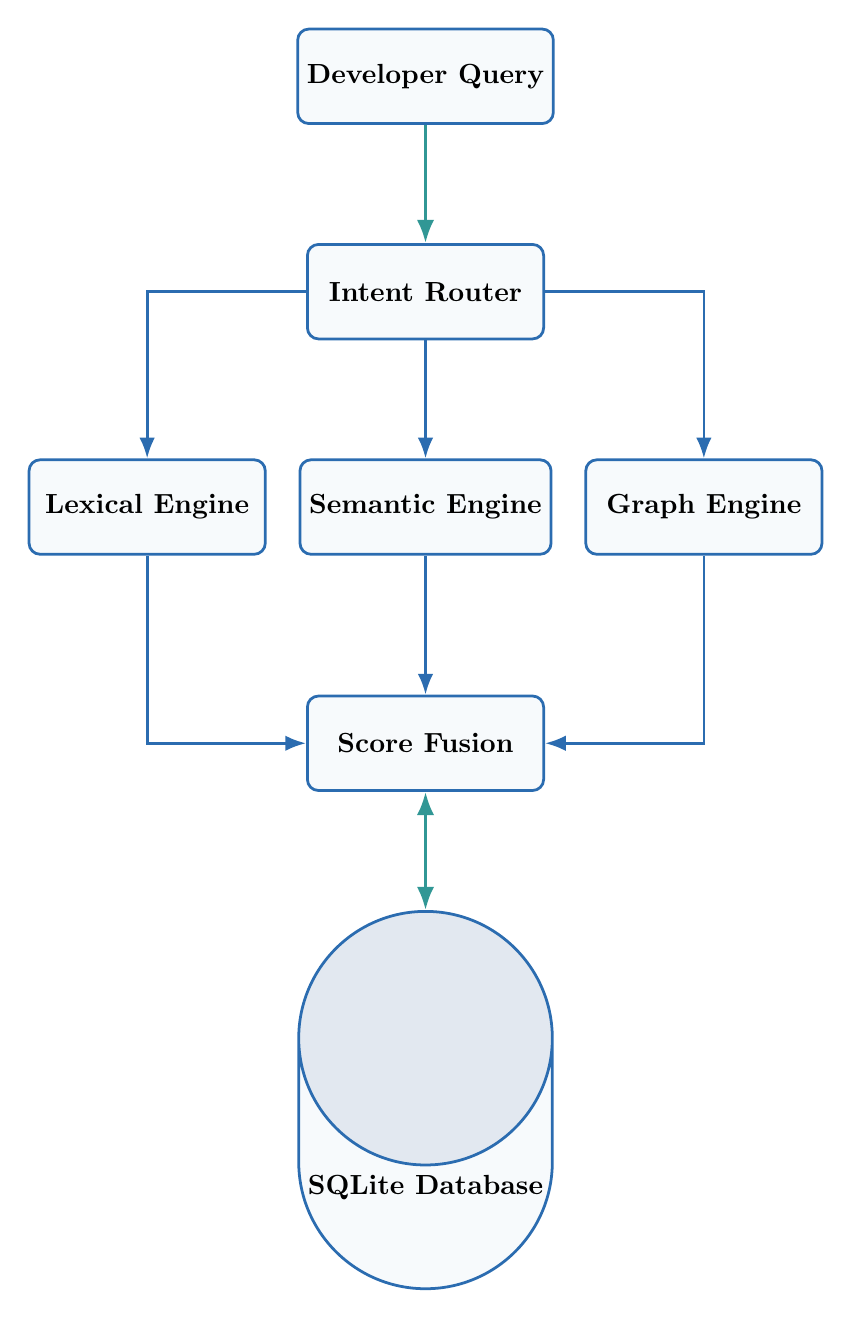
\begin{tikzpicture}[node distance=2cm, auto, >=Latex]
        \tikzstyle{block} = [rectangle, draw=secondary, fill=lightbg, rounded corners, minimum width=3cm, minimum height=1.2cm, text centered, line width=1pt]
        \tikzstyle{database} = [cylinder, cylinder uses custom fill, cylinder body fill=lightbg, cylinder end fill=border, draw=secondary, shape border rotate=90, minimum width=2.5cm, minimum height=1.5cm, text centered, line width=1pt]
        
        \node [block] (input) {\bfseries Developer Query};
        \node [block, below=1.5cm of input] (router) {\bfseries Intent Router};
        \node [block, below left=1.5cm and 0.5cm of router] (fts) {\bfseries Lexical Engine};
        \node [block, below=1.5cm of router] (onnx) {\bfseries Semantic Engine};
        \node [block, below right=1.5cm and 0.5cm of router] (graph) {\bfseries Graph Engine};
        \node [block, below=4.5cm of router] (fusion) {\bfseries Score Fusion};
        \node [database, below=1.5cm of fusion] (sqlite) {\bfseries SQLite Database};
        
        \path [draw, ->, line width=1.2pt, color=accent] (input) -- (router);
        \path [draw, ->, line width=1pt, color=secondary] (router) -| (fts);
        \path [draw, ->, line width=1pt, color=secondary] (router) -- (onnx);
        \path [draw, ->, line width=1pt, color=secondary] (router) -| (graph);
        \path [draw, ->, line width=1pt, color=secondary] (fts) |- (fusion);
        \path [draw, ->, line width=1pt, color=secondary] (onnx) -- (fusion);
        \path [draw, ->, line width=1pt, color=secondary] (graph) |- (fusion);
        \path [draw, <->, line width=1.2pt, color=accent] (fusion) -- (sqlite);
    \end{tikzpicture}
    
    \vfill
    {\large \bfseries \color{primary} Version 1.0.0}\\[0.2cm]
    {\large \color{accent} Technical Architecture \& Consolidated Plan}\\[1cm]
\end{titlepage}

\newpage
\tableofcontents
\newpage

% ============================================================
% SECTION 1: EXECUTIVE SUMMARY
% ============================================================
\section{Executive Summary}
This document outlines the architecture for \textbf{MyRAG}, a lightweight, fully offline Retrieval-Augmented Generation (RAG) system optimized specifically for Vite + React projects. The system is designed to provide high-precision code retrieval and understanding under a strict operating memory constraint of \textbf{20 megabytes of RAM} per indexed project.

Unlike general-purpose assistants, this system maps the structural features of React (such as custom hooks, route maps, components, state hooks, and context providers) and fuses them with lexical and semantic indices. The result is a robust, localized search pipeline that processes queries, traces dependencies, and analyzes system modifications entirely on the user's local machine.

---

% ============================================================
% SECTION 2: THE 20MB MEMORY BUDGET
% ============================================================
\section{Memory Optimization \& RAM Budget}
The core constraint of this architecture is maintaining a minimal memory footprint. The diagram below illustrates how the strict 20MB memory limit is allocated among the runtime processes.

\subsection{Memory Allocation Visual Map}
\begin{center}
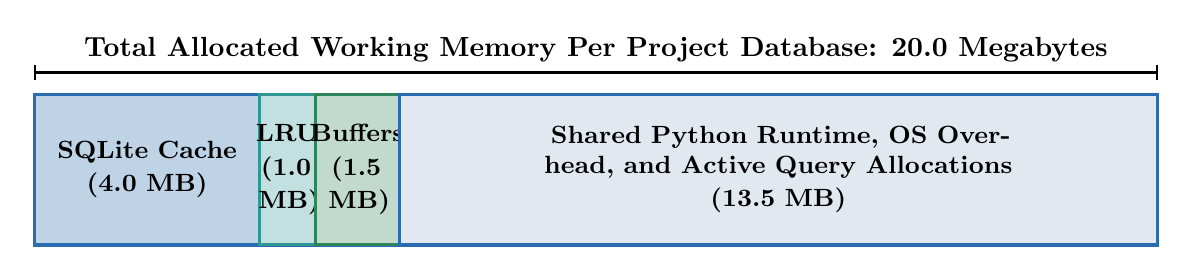
\begin{tikzpicture}[scale=0.95]
    % Draw the total budget bar
    \draw[draw=secondary, fill=lightbg, line width=1.5pt] (0,0) rectangle (15,2);
    
    % Segments representing allocations
    \draw[fill=secondary!30, draw=secondary, line width=1pt] (0,0) rectangle (3,2) node[pos=.5, text width=2.8cm, align=center] {\small \bfseries SQLite Cache\\(4.0 MB)};
    \draw[fill=accent!30, draw=accent, line width=1pt] (3,0) rectangle (3.75,2) node[pos=.5, text width=0.8cm, align=center] {\small \bfseries LRU\\(1.0 MB)};
    \draw[fill=success!30, draw=success, line width=1pt] (3.75,0) rectangle (4.875,2) node[pos=.5, text width=1.2cm, align=center] {\small \bfseries Buffers\\(1.5 MB)};
    \draw[fill=border, draw=secondary, line width=1pt] (4.875,0) rectangle (15,2) node[pos=.5, text width=9.5cm, align=center] {\small \bfseries Shared Python Runtime, OS Overhead, and Active Query Allocations\\(13.5 MB)};
    
    % Capping brackets and labels
    \draw[line width=1.2pt] (0, 2.3) -- (15, 2.3) node[midway, above] {\bfseries Total Allocated Working Memory Per Project Database: 20.0 Megabytes};
    \draw[line width=1pt] (0, 2.2) -- (0, 2.4);
    \draw[line width=1pt] (15, 2.2) -- (15, 2.4);
\end{tikzpicture}
\end{center}

\subsection{Subsystem Budget Rationale}
\begin{itemize}
    \item \textbf{SQLite Page Cache Limit (4.0 MB):} Capped strictly on connection setup to prevent the database page cache from scaling dynamically with the database size.
    \item \textbf{Vector LRU Cache (1.0 MB):} Temporarily stores recently dequantized float32 vectors in memory. If a new query requests vectors, older entries are evicted to keep vector-associated memory bounded.
    \item \textbf{Graph Traversal Buffers (0.5 MB):} Designed to support active Breadth-First Search (BFS) queues. The buffer keeps only the active frontier nodes in memory during path traversal, keeping search operations extremely light.
    \item \textbf{Active Working Sets (1.0 MB):} Buffers active textual queries, lexical matched candidate lists, and query response JSON builders.
\end{itemize}

---

% ============================================================
% SECTION 3: THE PIPELINES
% ============================================================
\section{System Pipelines \& Data Flow}
MyRAG divides responsibilities into three logical pathways: the **Indexing Pipeline**, the **Retrieval Pipeline**, and the **Reasoning Pipeline**.

\subsection{The Indexing Pipeline Data Flow}
The indexing pipeline extracts code modules, chunks them semantically, and stores them in the localized SQLite database.

\begin{center}
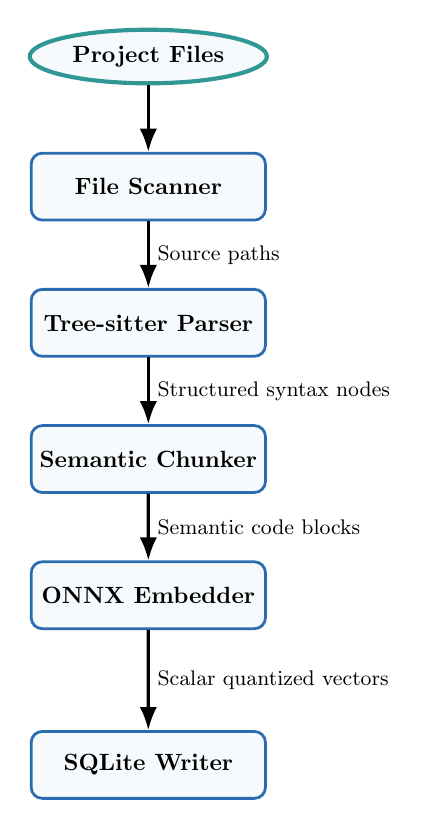
\begin{tikzpicture}[node distance=1.5cm, auto, >=Latex, scale=0.85, every node/.style={transform shape}]
    \tikzstyle{process} = [rectangle, draw=secondary, fill=lightbg, rounded corners, minimum width=3.5cm, minimum height=1cm, text centered, line width=1pt]
    \tikzstyle{io} = [ellipse, draw=accent, fill=lightbg, minimum width=2.5cm, minimum height=0.8cm, text centered, line width=1.5pt]
    
    \node [io] (start) {\bfseries Project Files};
    \node [process, below=1cm of start] (scanner) {\bfseries File Scanner};
    \node [process, below=1cm of scanner] (parser) {\bfseries Tree-sitter Parser};
    \node [process, below=1cm of parser] (chunker) {\bfseries Semantic Chunker};
    \node [process, below=1cm of chunker] (vectorizer) {\bfseries ONNX Embedder};
    \node [process, below=1.5cm of vectorizer] (writer) {\bfseries SQLite Writer};
    
    \path [draw, ->, line width=1.2pt] (start) -- (scanner);
    \path [draw, ->, line width=1.2pt] (scanner) -- node[right] {\small Source paths} (parser);
    \path [draw, ->, line width=1.2pt] (parser) -- node[right] {\small Structured syntax nodes} (chunker);
    \path [draw, ->, line width=1.2pt] (chunker) -- node[right] {\small Semantic code blocks} (vectorizer);
    \path [draw, ->, line width=1.2pt] (vectorizer) -- node[right] {\small Scalar quantized vectors} (writer);
\end{tikzpicture}
\end{center}

\newpage

\subsection{The Retrieval Pipeline Data Flow}
The retrieval pipeline uses three signals to match a natural language query with the most relevant code chunks.

\begin{center}
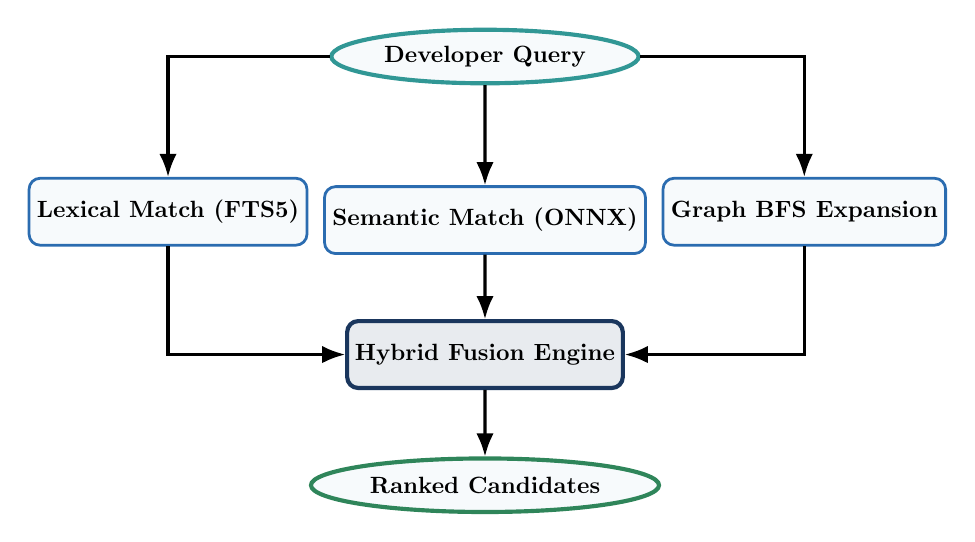
\begin{tikzpicture}[node distance=1.5cm, auto, >=Latex, scale=0.85, every node/.style={transform shape}]
    \tikzstyle{query} = [ellipse, draw=accent, fill=lightbg, minimum width=3cm, minimum height=0.8cm, text centered, line width=1.5pt]
    \tikzstyle{engine} = [rectangle, draw=secondary, fill=lightbg, rounded corners, minimum width=3.5cm, minimum height=1cm, text centered, line width=1.0pt]
    \tikzstyle{combiner} = [rectangle, draw=primary, fill=primary!10, rounded corners, minimum width=4cm, minimum height=1cm, text centered, line width=1.5pt]
    \tikzstyle{output} = [ellipse, draw=success, fill=lightbg, minimum width=3cm, minimum height=0.8cm, text centered, line width=1.5pt]
    
    \node [query] (q) {\bfseries Developer Query};
    
    \node [engine, below left=1.5cm and 1cm of q] (fts) {\bfseries Lexical Match (FTS5)};
    \node [engine, below=1.5cm of q] (onnx) {\bfseries Semantic Match (ONNX)};
    \node [engine, below right=1.5cm and 1cm of q] (graph) {\bfseries Graph BFS Expansion};
    
    \node [combiner, below=3.5cm of q] (fuse) {\bfseries Hybrid Fusion Engine};
    \node [output, below=1cm of fuse] (res) {\bfseries Ranked Candidates};
    
    \path [draw, ->, line width=1.2pt] (q) -| (fts);
    \path [draw, ->, line width=1.2pt] (q) -- (onnx);
    \path [draw, ->, line width=1.2pt] (q) -| (graph);
    
    \path [draw, ->, line width=1.2pt] (fts) |- (fuse);
    \path [draw, ->, line width=1.2pt] (onnx) -- (fuse);
    \path [draw, ->, line width=1.2pt] (graph) |- (fuse);
    
    \path [draw, ->, line width=1.2pt] (fuse) -- (res);
\end{tikzpicture}
\end{center}

---

% ============================================================
% SECTION 4: DATABASE SCHEMAS
% ============================================================
\section{Database Design}
The relational schema is mapped onto a single, zero-dependency SQLite database. The table below outlines the responsibilities of each database table.

\subsection{Database Tables Summary}
\begin{table}[h!]
\centering
\begin{tabular}{llp{7.5cm}}
\toprule
\bfseries Table Name & \bfseries Primary Key & \bfseries Description \& Relationships \\
\midrule
\rowcolor{lightbg}
\bfseries files & Path ID & Holds file hashes, path strings, and scan timestamps. \\
\bfseries chunks & Chunk ID & Stores functional code blocks, line bounds, and metadata tags. \\
\rowcolor{lightbg}
\bfseries fts\_chunks & Virtual ID & Virtual table for FTS5 lexical indexes using Porter-stemming. \\
\bfseries symbols & Auto-increment & Maps declared hooks, helpers, and components for symbol resolution. \\
\rowcolor{lightbg}
\bfseries embeddings & Chunk ID & Stores scalar quantized 8-bit embedding vectors alongside scale factors. \\
\bfseries graph\_edges & Edge ID & Maps imports, rendering connections, state usage, and custom hook calls. \\
\rowcolor{lightbg}
\bfseries routes & Route ID & Stores React Router paths, wrappers, and lazy-loading states. \\
\bfseries api\_calls & Call ID & Logs dynamic endpoints and fetch client models. \\
\bottomrule
\end{tabular}
\caption{MyRAG Schema Summary}
\end{table}

---

% ============================================================
% SECTION 5: INTENT AND SCORE FUSION MATRIX
% ============================================================
\section{Intent-Aware Retrieval Weights}
Weights assigned to each of the three signals are dynamically adjusted based on the query's detected intent.

\subsection{Strategy Weight Table}
\begin{table}[h!]
\centering
\begin{tabular}{lccccl}
\toprule
\bfseries Query Intent Category & \bfseries Lexical Weight & \bfseries Semantic Weight & \bfseries Graph Weight & \bfseries BFS Depth & \bfseries Primary Edge Target \\
\midrule
\rowcolor{lightbg}
\textbf{SYMBOL\_LOOKUP} & 0.70 & 0.20 & 0.10 & 1 & Calls, Hook usage \\
\textbf{ARCHITECTURE} & 0.20 & 0.30 & 0.50 & 3 & All structural edges \\
\rowcolor{lightbg}
\textbf{MODIFICATION} & 0.30 & 0.50 & 0.20 & 2 & Imports, Providers \\
\textbf{DEBUGGING} & 0.40 & 0.40 & 0.20 & 2 & State mutations, Calls \\
\rowcolor{lightbg}
\textbf{RERENDER\_ANALYSIS} & 0.30 & 0.40 & 0.30 & 2 & Render tree, Hook calls \\
\textbf{ROUTE\_TRACING} & 0.20 & 0.20 & 0.60 & 4 & Route nodes, Imports \\
\rowcolor{lightbg}
\textbf{IMPACT\_ANALYSIS} & 0.20 & 0.20 & 0.60 & 3 & Incoming connections \\
\bottomrule
\end{tabular}
\caption{Retrieval Strategy Weights by Intent}
\end{table}

---

% ============================================================
% SECTION 6: GRAPH RELATIONSHIP MODELING
% ============================================================
\section{Graph Representation}
The graph engine maps structural dependencies across Vite + React applications. The diagram below shows how different edges represent structural connections within the codebase.

\subsection{Logical Dependency Hierarchy}
\begin{center}
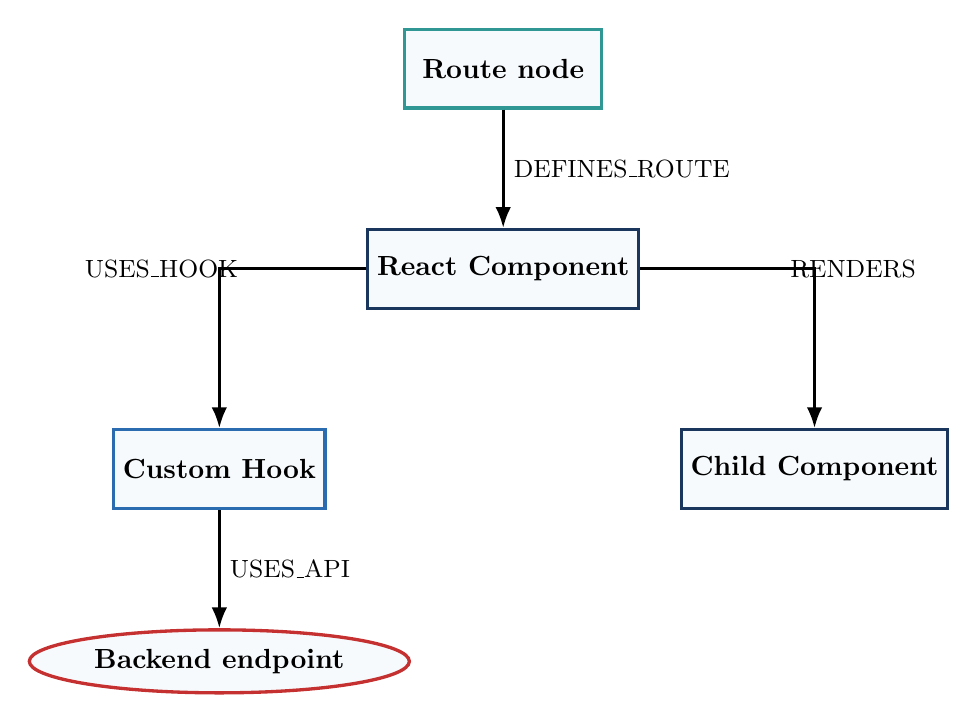
\begin{tikzpicture}[node distance=2.2cm, auto, >=Latex]
    \tikzstyle{route} = [rectangle, draw=accent, fill=lightbg, line width=1.2pt, minimum width=2.5cm, minimum height=1cm, text centered]
    \tikzstyle{comp} = [rectangle, draw=primary, fill=lightbg, line width=1.2pt, minimum width=2.5cm, minimum height=1cm, text centered]
    \tikzstyle{hook} = [rectangle, draw=secondary, fill=lightbg, line width=1.2pt, minimum width=2.5cm, minimum height=1cm, text centered]
    \tikzstyle{api} = [ellipse, draw=alert, fill=lightbg, line width=1.2pt, minimum width=2cm, minimum height=0.8cm, text centered]
    
    \node [route] (r) {\bfseries Route node};
    \node [comp, below=1.5cm of r] (c) {\bfseries React Component};
    \node [hook, below left=1.5cm and 0.5cm of c] (h) {\bfseries Custom Hook};
    \node [comp, below right=1.5cm and 0.5cm of c] (ch) {\bfseries Child Component};
    \node [api, below=1.5cm of h] (a) {\bfseries Backend endpoint};
    
    \path [draw, ->, line width=1pt] (r) -- node[right] {\small DEFINES\_ROUTE} (c);
    \path [draw, ->, line width=1pt] (c) -| node[left, pos=0.4] {\small USES\_HOOK} (h);
    \path [draw, ->, line width=1pt] (c) -| node[right, pos=0.4] {\small RENDERS} (ch);
    \path [draw, ->, line width=1pt] (h) -- node[right] {\small USES\_API} (a);
\end{tikzpicture}
\end{center}

\newpage

% ============================================================
% SECTION 7: SCALAR QUANTIZATION PROCESS
% ============================================================
\section{Vector Scalar Quantization Process}
Standard float32 vectors are converted into highly compressed 8-bit integers to minimize database footprint. The diagram below illustrates how values are mapped into the quantized space.

\subsection{Quantization Transform Flow}
\begin{center}
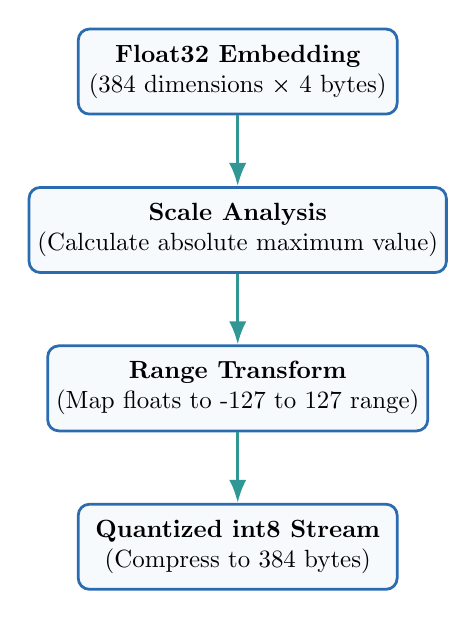
\begin{tikzpicture}[node distance=2cm, auto, >=Latex, scale=0.9, every node/.style={transform shape}]
    \tikzstyle{qstep} = [rectangle, draw=secondary, fill=lightbg, rounded corners, minimum width=4.5cm, minimum height=1.2cm, text centered, align=center, line width=1pt]
    
    \node [qstep] (s1) {\bfseries Float32 Embedding\\(384 dimensions × 4 bytes)};
    \node [qstep, below=1cm of s1] (s2) {\bfseries Scale Analysis\\(Calculate absolute maximum value)};
    \node [qstep, below=1cm of s2] (s3) {\bfseries Range Transform\\(Map floats to -127 to 127 range)};
    \node [qstep, below=1cm of s3] (s4) {\bfseries Quantized int8 Stream\\(Compress to 384 bytes)};
    
    \path [draw, ->, line width=1.2pt, color=accent] (s1) -- (s2);
    \path [draw, ->, line width=1.2pt, color=accent] (s2) -- (s3);
    \path [draw, ->, line width=1.2pt, color=accent] (s3) -- (s4);
\end{tikzpicture}
\end{center}

---

% ============================================================
% SECTION 8: 20MB RAM ACHIEVEMENT STRATEGY
% ============================================================
\section{Achieving the 20MB RAM Target}
Maintaining an operational memory limit of under 20 megabytes per project requires strict control over how data is processed, indexed, and stored. The pipeline implements several conceptual strategies to achieve this:

\subsection{SQLite Connection Page Caps}
Standard database engines often allocate dynamic page caches that scale alongside the size of the database. To prevent this, the connection adapter restricts the SQLite page cache pool to exactly 4.0 megabytes. This ensures that no matter how large the database grows on disk, the database page-caching layer will never exceed this allocation boundary.

\subsection{Lazy Embedding Matrix Projection}
Traditional vector search engines (such as FAISS or HNSW indices) load the entire embedding matrix directly into memory to support rapid distance calculations. For hundreds of code chunks, this results in significant RAM consumption. 

MyRAG achieves its footprint by keeping the entire vector space on disk within a SQLite database file, stored as binary BLOBs. During a query, the system performs a two-tier retrieval:
\begin{enumerate}
    \item A fast lexical search (using the SQLite FTS5 index) acts as a filter, returning only the top 50 candidate chunks.
    \item The system then lazy-loads only the 50 corresponding quantized embedding BLOBs from disk into RAM.
    \item Cosine similarity is calculated only on these 50 candidates, keeping vector-related memory allocations under 20 kilobytes.
\end{enumerate}

\subsection{Dequantized Vector LRU Eviction}
To prevent memory leaks and dynamic heap growth during sequential queries, dequantized float32 vectors are managed inside a dedicated Least Recently Used (LRU) cache. This cache is configured with a strict ceiling of 1.0 megabyte. Once this threshold is reached, older decoded vectors are immediately evicted, keeping active vector allocations fully bounded.

\subsection{Immediate AST Garbage Collection}
Abstract Syntax Trees (ASTs) generated during parsing can occupy a large amount of heap memory if kept in active memory. MyRAG addresses this by processing files sequentially:
\begin{itemize}
    \item The system loads and parses a single file to extract metadata (such as hook references, component identifiers, and import targets).
    \item These metrics are immediately written to the database.
    \item The AST representation is deleted, freeing the C-level memory before the next file is processed.
\end{itemize}

\subsection{Bounded Traversal Frontiers}
Rather than loading the complete dependency graph into memory, MyRAG performs structural path traversals (like BFS and DFS) directly via indexed SQLite self-joins. The traversal queue only holds active frontier node IDs in memory, keeping traversal memory usage under 10 kilobytes even for deep path resolutions.

---

% ============================================================
% SECTION 9: SELECTED TECHNOLOGIES \& RATIONALE
% ============================================================
\section{Selected Technology Stack}
The stack has been selected to ensure absolute local performance, a minimal memory footprint, and high parsing precision without external runtime dependencies.

\subsection{Technology Stack Summary}
\begin{table}[h!]
\centering
\begin{tabular}{llp{7.5cm}}
\toprule
\bfseries Technology & \bfseries Operational Footprint & \bfseries Technical Rationale \\
\midrule
\rowcolor{lightbg}
\textbf{Python} & $\sim$10.0 MB core runtime & Provides mature bindings for the ONNX runtime, robust file handling, and simple integration with local execution layers. \\
\textbf{SQLite} & $\le$4.0 MB page cache & Serverless, self-contained database engine. Features a built-in FTS5 extension that provides fast lexical indexing with Porter-stemming. \\
\rowcolor{lightbg}
\textbf{Tree-Sitter} & Temporary C-level heap & Fast incremental parser that handles malformed or draft code gracefully, ensuring reliable React AST extraction. \\
\textbf{ONNX Runtime} & $\sim$30.0 MB shared globally & Highly optimized CPU execution environment. Enables in-process loading of the compressed 22MB MiniLM model. \\
\rowcolor{lightbg}
\textbf{FastAPI} & $\le$2.5 MB runtime memory & Ultra-lightweight asynchronous web gateway that exposes search and dependency routing endpoints. \\
\textbf{Watchdog} & Negligible background load & Uses native operating system filesystem event wrappers to monitor file changes with built-in event debouncing. \\
\bottomrule
\end{tabular}
\caption{MyRAG Technology Stack Analysis}
\end{table}

\subsection{Stack Synergies}
The synergy between \textbf{SQLite} and the \textbf{ONNX Runtime} is key to achieving the system's performance goals. By using FTS5 as a fast candidate filter, the system avoids loading the entire embedding matrix into memory, allowing the ONNX vector calculations to run in a highly bounded environment. This combination delivers fast query performance while staying well within the target memory constraints.

---

% ============================================================
% SECTION 10: CONCLUSION
% ============================================================
\section{Conclusion}
This architectural blueprint provides a memory-efficient solution for offline RAG on web codebases. By prioritizing targeted chunking, lazy vector loads, in-memory traversal, and scalar quantization, the pipeline delivers accurate context while staying under a strict 20MB RAM ceiling.

\end{document}
